\documentclass{standalone}
\usepackage{tikz}
\usepackage{ctex,siunitx}
\setCJKmainfont{Noto Serif CJK SC}
\usepackage{tkz-euclide}
\usepackage{amsmath}
\usetikzlibrary{patterns, calc}
\usetikzlibrary {decorations.pathmorphing, decorations.pathreplacing, decorations.shapes,}

\begin{document}
\small
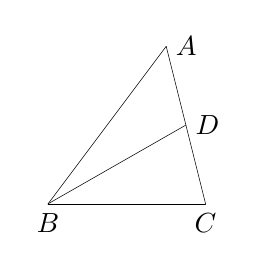
\begin{tikzpicture}[>=stealth,scale=1]
  \tkzSetUpPoint[fill=black]
  % \useasboundingbox(-1,-0.75)rectangle(3.7,1.4);
  \tkzDefPoints{0/0/B, 2/0/C, 1.5/2/A}
  \tkzDefMidPoint(A,C) \tkzGetPoint{D}
  \tkzDrawSegments(B,C A,B A,C B,D)
  \tkzLabelPoints[below](B,C)
  \tkzLabelPoints[right](A,D)	
\end{tikzpicture}
\end{document}